%%%%%%%%%%%%%%%%%%%%%%%%%%%%%%%%%%%%%%%%%%%%%%%%%%%%%%%%%%%%%%%%%%%%%%%%%%%%%
%%%
%%% File: thesis.tex, version 1.9, May 2015
%%%
%%% =============================================
%%% This file contains a template that can be used with the package
%%% cs.sty and LaTeX2e to produce a thesis that meets the requirements
%%% of the Computer Science Department from the Technical University of Cluj-Napoca
%%%%%%%%%%%%%%%%%%%%%%%%%%%%%%%%%%%%%%%%%%%%%%%%%%%%%%%%%%%%%%%%%%%%%%%%%%%%%

\documentclass[12pt,a4paper,twoside]{report}         
\usepackage{cs}              
\usepackage{times}
\usepackage{graphicx}
\usepackage{latexsym}
\usepackage{amsmath,amsbsy}
\usepackage{amssymb}
\usepackage[matrix,arrow]{xy}
\usepackage[T1]{fontenc}
\usepackage{ae,aecompl}
%\usepackage{shortcut} %definitii pentru diacritice; 
\usepackage{amstext}
\usepackage{graphics}
\usepackage[T1]{fontenc}
\usepackage{ae,aecompl}
\usepackage{algorithm}
%\usepackage{algorithmic}
\usepackage{color}
\usepackage{color}

% \mastersthesis
\diplomathesis
% \leftchapter
\centerchapter
% \rightchapter
\singlespace
% \oneandhalfspace
% \doublespace

\renewcommand{\thesisauthor}{Firstname LASTNAME}    %% Your name.
\renewcommand{\thesismonth}{June}     %% Your month of graduation.
\renewcommand{\thesisyear}{2015}      %% Your year of graduation.
\renewcommand{\thesistitle}{LICENSE THESIS TITLE} 
\renewcommand{\thesissupervisor}{scientific title Firstname LASTNAME}
\newcommand{\department}{\bf FACULTY OF AUTOMATION AND COMPUTER SCIENCE\\
COMPUTER SCIENCE DEPARTMENT}
\newcommand{\thesis}{LUCRARE DE LICEN'T'A}
\newcommand{\utcnlogo}{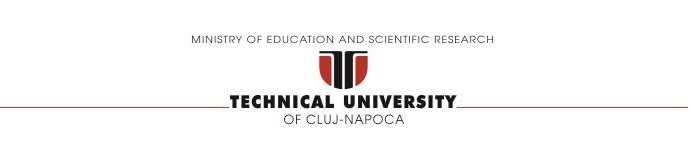
\includegraphics[width=15cm]{img/tucn.jpg}}

\newcommand{\uline}[1]{\rule[0pt]{#1}{0.4pt}}
%\renewcommand{\thesisdedication}{P\u{a}rin\c{t}ilor mei}

\begin{document}
%\frontmatter
%\pagestyle{headings}

\newenvironment{definition}[1][Defini\c{t}ie.]{\begin{trivlist}
\item[\hskip \labelsep {\bfseries #1}]}{\end{trivlist}}



%\thesistitle                    %% Generate the title page.
%\authordeclarationpage                %% Generate the declaration page.

\pagenumbering{arabic}
\setcounter{page}{4}



\begin{center}
\utcnlogo

\department

\vspace{4cm}

{\bf \thesistitle} %LICENSE THESIS TITLE}

\vspace{1.5cm}

LICENSE THESIS

\vspace{6cm}

Graduate: {\bf Firstname LASTNAME} 

Supervisor: {\bf \thesissupervisor}

\vspace{3cm}
{\bf \thesisyear}
\end{center}

\thispagestyle{empty}
\newpage

\begin{center}
\utcnlogo

\department

\end{center}
\vspace{0.5cm}

%\begin{small}
\begin{tabular}{p{7cm}p{8cm}}
 %\hspace{-1cm}& APPROVED,\\
 \hspace{-1cm}DEAN, & HEAD OF DEPARTMENT,\\
\hspace{-1cm}{\bf Prof. dr. eng. Liviu MICLEA} & {\bf Prof. dr. eng. Rodica POTOLEA}\\  
\end{tabular}
 
\vspace{2cm}

\begin{center}
Graduate: {\bf \thesisauthor}

\vspace{1cm}

{\bf \thesistitle}
\end{center}

\vspace{1cm}

\begin{enumerate}
 \item {\bf Project proposal:} {\it Short description of the license thesis and initial data}
\item {\bf Project contents:} {\it (enumerate the main component parts) Presentation page, advisor's evaluation, title of chapter 1, title of chapter 2, ..., title of chapter n, bibliography, appendices.}
\item {\bf Place of documentation:} {\it Example}: Technical University of Cluj-Napoca, Computer Science Department
\item {\bf Consultants:}
\item {\bf Date of issue of the proposal:} November 1, 2014
\item {\bf Date of  delivery:} June 18, 2015 {\it (the date when the document is submitted)}
  \end{enumerate}
\vspace{1.2cm}

\hspace{6cm} Graduate: \uline{6cm} 

\vspace{0.5cm}
\hspace{6cm} Supervisor: \uline{6cm} 
%\end{small}

\thispagestyle{empty}


\newpage
$ $
%\begin{center}
%\utcnlogo

%\department
%\end{center}

\thispagestyle{empty}
\newpage

\begin{center}
\utcnlogo

\department
\end{center}

\vspace{0.5cm}

\begin{center}
{\bf
Declara\c{t}ie pe proprie r\u{a}spundere privind\\ 
autenticitatea lucr\u{a}rii de licen\c{t}\u{a}}
\end{center}
\vspace{1cm}



Subsemnatul(a) \\
\uline{14.8cm}, 
legitimat(\u{a}) cu \uline{4cm} seria \uline{3cm} nr. \uline{4cm}\\
CNP \uline{9cm}, autorul lucr\u{a}rii \uline{2.8cm}\\
\uline{16cm}\\
\uline{16cm}\\
elaborat\u{a} \^{\i}n vederea sus\c{t}inerii examenului de finalizare a studiilor de licen\c{t}\u{a} la Facultatea de Automatic\u{a} \c{s}i Calculatoare, Specializarea \uline{7cm} din cadrul Universit\u{a}\c{t}ii Tehnice din Cluj-Napoca, sesiunea \uline{4cm} a anului universitar \uline{3cm}, declar pe proprie r\u{a}spundere, c\u{a} aceast\u{a} lucrare este rezultatul propriei activit\u{a}\c{t}i intelectuale, pe baza cercet\u{a}rilor mele \c{s}i pe baza informa\c{t}iilor ob\c{t}inute din surse care au fost citate, \^{\i}n textul lucr\u{a}rii \c{s}i \^{\i}n bibliografie.

Declar, c\u{a} aceast\u{a} lucrare nu con\c{t}ine por\c{t}iuni plagiate, iar sursele bibliografice au fost folosite cu 
respectarea legisla\c{t}iei rom\^{a}ne \c{s}i a conven\c{t}iilor interna\c{t}ionale privind drepturile de autor.

Declar, de asemenea, c\u{a} aceast\u{a} lucrare nu a mai fost prezentat\u{a} \^{\i}n fa\c{t}a unei alte comisii de examen de licen\c{t}\u{a}.

\^{I}n cazul constat\u{a}rii ulterioare a unor declara\c{t}ii false, voi suporta sanc\c{t}iunile administrative, respectiv, \emph{anularea examenului de licen\c{t}\u{a}}.

\vspace{1.5cm}

Data \hspace{8cm} Nume, Prenume

\vspace{0.5cm}

\uline{3cm} \hspace{5cm} \uline{5cm}

\vspace{1cm}
\hspace{9.4cm}Semn\u{a}tura

\thispagestyle{empty}

\newpage


%\listoftables
%\listoffigures

%\clearpage 
%\newpage

%\begin{comment}
{\color{red}{\bf De citit \^{\i}nainte} (aceast\u{a} pagin\u{a} se va elimina din versiunea final\u{a})}:
\begin{enumerate}
 \item Cele trei pagini anterioare (foaie de cap\u{a}t, foaie sumar, declara\c{t}ie) se vor lista pe foi separate (nu fa\c{t}\u{a}-verso), fiind incluse \^{\i}n lucrarea listat\u{a}. 
 Foaia de sumar (a doua) necesit\u{a} semn\u{a}tura absolventului, respectiv a coordonatorului.
 Pe declara\c{t}ie se trece data c\^{a}nd se pred\u{a} lucrarea la secretarii de comisie.
 \item Pe foaia de cap\u{a}t, se va trece corect titulatura cadrului didactic \^{\i}ndrum\u{a}tor, \^{\i}n englez\u{a} (consulta\c{t}i pagina de unde a\c{t}i desc\u{a}rcat acest document pentru lista cadrelor didactice cu titulaturile lor).
 \item Documentul curent {\bf nu} a fost creat \^{\i}n MS Office. E posibil sa fie mici diferen\c{t}e de formatare. 
\item Cuprinsul \^{\i}ncepe pe pagina nou\u{a}, impar\u{a} (dac\u{a} se face listare fa\c{t}\u{a}-verso), prima pagin\u{a} din capitolul \emph{Introducere} tot a\c{s}a, fiind numerotat\u{a} cu 1. % Pentru actualizarea cuprinsului, click dreapta pe cuprins (zona cuprinsului va apare cu gri), Update field-$>$Update entire table.
\item E recomandat s\u{a} vizualiza\c{t}i acest document \c{s}i \^{\i}n timpul edit\u{a}rii lucr\u{a}rii. % după ce activaţi vizualizarea simbolurilor ascunse de formatare (apăsaţi simbolul  din Home/Paragraph).
\item Fiecare capitol \^{\i}ncepe pe pagin\u{a} nou\u{a}. % datorită simbolului ascuns Section Break (Next Page) care este deja introdus la capitolul precedent. Dacă ştergeţi din greşeală simbolul, se reintroduce (Page Layout -> Breaks).
\item Folosi\c{t}i stilurile predefinite (Headings, Figure, Table, Normal, etc.)
\item Marginile la pagini nu se modific\u{a}.
\item Respecta\c{t}i restul instruc\c{t}iunilor din fiecare capitol.
\end{enumerate}
 
%\end{comment}

\newpage

\tableofcontents
\newpage



\chapter{Introduction - Project Context}
\pagestyle{headings}
{\color{red}{must be about 3 pages}}

Optical flow does not originate in computer vision, but in psychology, psychophysics. One of th most influential man in this field is J.J. Gibson. He was the one who asked "How do we see the world around us?" and answered in his many publications around the '50s. In his book\cite{gibson1950perception}, Gibson explains how the stimuli are correlated to the perception of motion. 
We perceive the motion in 2D as a projection of the 3D world. This projection is nothing else but the light reflected from the environment, hitting our retina, referred as the optical array. In a analytical context, he defines the movement for a perception. Each element is detected and associated a pair of coordinates. Then each element has a motion descriptor as either a pair of elements or a speed and direction component, in successive moments in time. 

As the nature is the grand engineer, the same model is taken in computer vision for computing the optical flow. The changes in the optical array are stocked in a series of frames. The perceived image is a 2D array of pixels. Each pixel is a element in the movement. An accurate and robust flow estimation implies an approximation for each pixel of the frame. The result will be a vector field indicating the direction and that each pixel takes between frames.
 






\chapter{Project Objectives and Specifications}
{\color{red}{must be about 6 pages}}

Describe the proper theme (as a research/design proposal, clearly formulated, with clear objectives, and some explanatory figures).

Stretches over about 10\% of the paper.

\section{Optical Flow Formulations}
\section{Solving the Optical Flow System}

\chapter{Bibliographic research}


{\color{red}{must be about 9 pages}}

Optical Flow problem is an old subject in computer vision. The fundamental method for robust optical flow, referenced in over $10000$ articles up to the newest, was published in 1980, by Horn and Schunch ~\cite{HSOpticalFlow}. They define the optical flow as
\begin{quote}
"the distribution of apparent velocities of movement in an image."
\end{quote}
and state the problem as a minimization of a squared penalty function from the brightness constraint and the smoothness constraint.

Based on this approach, many other algorithms were published. All this formulations, spatially-discrete, derived from Horn-Scunk are referred in literature as "clasics"~\cite{sun2010,QAnalysis}. They all combine a data term and a spatial term, and apply an optimization procedure to minimize the function. 

Another heavily cited article was published in the same year by Lucas and Kanade ~\cite{lucas1981}. This approach solves the problem as a sum of squared differences, and proposes a coarse-to-fine solution for large displacements. As stated in chapter 3 from~\cite{mitiche2014computer} the main weakness of this algorithm compared to Horn Schunk 's is the lack of regularization.
 


\section{First Approaches}

Differential techniques compute the optical flow trough spatio-temporal derivatives.
Most algorithms start from the brightness constraint and from a Taylor expansion, obtaining the gradient constraint. Details of the numerical scheme of this chapter will be furthered discussed in \ref{BrightnessConstr}

Then, for a complete formulation of the problem, a regularization term is needed. In the first chapter of~\cite{wedel2011stereo}, the algorithms are classified in two categories, depending on the regularization term, variational and feature-based, meaning it does or does not depend on neighbouring pixels' flow computations.
\subsection{Horn Schunk}
The first important formulation of te global optical flow was stated by Horn and Schunk in ~\cite{HSOpticalFlow}. They started from the brightness constraint, a moving point does not change its brightness in time. From this constraint results the temporal derivative of the brightness of a sequence is $0$. Then,  using multi-dimensional Euler-Lagrange equations, from the expansion of the derivative, optical flow  can be formulated in one equation as the data term. But the optical flow has two components, the horizontal flow, and the vertical flow. To solve this problem, another constraint is introduced, the spatial smoothness constrained. 

Smoothness constraint is a variational method, that means it takes into account flow solutions of neighbourhood pixels. By assuming a continuous flow, the neighbouring pixels should have similar velocities\cite{HSOpticalFlow}. Further, by applying the Laplacian operator on the flow, the result should be 0. By minimizing the Laplacian, the flow propagates on texureless objects.

By combining the two constraints, the results a convex energy function:
\begin{equation} \label{HSEq}
	\iint  ((\nabla I + I_t)^2 + \lambda(\left\Vert(\nabla u) \right\Vert_2^2 +\left\Vert(\nabla v) \right\Vert_2^2))dxdy
\end{equation}
where $\lambda$ is the smoothness term coefficient. Although, $\lambda$ is set to $100$ in the by Horn and Schunk, in the original version, some later analysis of the algorithm claim that if the coefficient ot set to values down to $0.5$ \cite{barron1994}, the algorithm yields better results. This proves that there is no optimal general value for $\lambda$, it should be approximated for each different set of images.

To solve the optical flow, the sum energy function \ref{HSEq} must be minimized. In order to obtain this minimization, variational calculus is applied. A set of two equations is obtained for the field.
Further, each vector is estimated with Gauss-Seidel iterations. This means that each point is computed from the anterior estimation. Gauss-Seidel iterations will be further discussed in \ref{GaussSeidel}


\subsection{Lucas Kanade}

Published in th same year with Horn and Schunk, the Lucas Kanade method, offers a local approach for solving the optical flow problem. 

It is also based on the brightness constraint, but the solution is local.
It is based on the least square fit.

\section{Coarse-to-fine}
Differential methods work well when the motion is small, about 1-2 pixels, because the differential techniques applied.
The coarse to fine method, as described by Lucas and Kanade in ~\cite{lucas1981} allows computation of greater displacements. for each image is computed a Gaussian Pyramid. Usually~\cite{sun2010}, the standard deviation used for the Gauss anti-aliasing filter is 
\begin{equation}
	\frac{1}{\sqrt{2d}}
\end{equation} where $d$ is the downsamplig factor.

The flow is estimated between each level, from the bottom, then warped to the next, finer level. At each finer scale, the residual motion is computed between the first image and the second image warped to the first. 

\subsection{Pyramid Height} \label{pyrHeight} About the height of the pyramid, it can vary from case to case. A general solution is to downsample until the top level has about 20-30 pixels in height or width~\cite{sun2010}. 

\subsection{Downsamplig}Also, they say the downsamplig factor should be $0.5$. most of the solutions take this value, but are some implementations that set the downsamplig factor at $0.8$. There should not be any difference in the result as the minimization function is convex. A good practice is considered to set it at $0.5$ \cite{sun2010}.



\subsection{Warping}In \cite{sun2010}, various methods are tested for wrapping. Their results state that good number for the warping times is 3. The difference in accuracy between 3 warps an 10 is insignificant.

\subsection{Interpolation technoques} Further, they compare the interpolation technique used before warping.
The diference between them is not significantly high, but they found that spline-based bicubic interpolation yields slightly better results.

\subsection{Drawbacks}In chapter 15 of ~\cite{fleet2006} the pyramid method is discussed. The author draws attention over the drawbacks of the coarse to fine methods. Each level's flow depends on its predecessor. If at some point in the computation of the velocities is erroneous, for example if aliasing or occlusions occur, it will be propagated up to the finest level.
 
\section{Solving the minimization problem}
Most of the formulation of the optical flow are stated as a minimization problem. If the penalty function is squared the solution can be achieved trough variational calculus. This is the case of the differential methods. For the L1 the classic methods do not apply  any more.
\paragraph{Gauss Seidel Iterations}

\section{$L^1$ techniques}
\subsection{Projected Proximal Point}
\subsection{Least Mixed Norm}

\section{Improvements}
\subsection{Low Pass Filter}

As stated above, most of the algorithms use a coarse to fine estimation, and, for each level, an iterative approximation is performed.
One of the downside of this approach is that if any outliers are present in the for at a lower level, this error will be propagated to all finer levels up to the final result, damaging the overall outcome of the algorithm.

In the papers comparing some of the existing algorithms, the implementations take a median filter somewhere in the algorithm.

In \cite{fleet2006}, the problem of aliasing is considered for bigger displacements, in th sampling procedure. The authors solve this problem by applying a blurring filer over the images, before computing the gradients of the images. From this they apply estimate the velocities for each level.

Also, in \cite{sun2010}, by analysing the best practices in solving the optical flow problem, it is proven that, if a median filter applied after each warp, th robustness and the accuracy of the algorithms is increased.
The robustness is a weak point of the differential methods. Outliers can completely throw off the energy function, especially in $L^2$ methods.
Their results compare different sizes of the median filter, and no filer of different algorithms. The best results are obtained with a $5 \times 5$ kernel. Also the accuracy of the results when no filter was applied is significantly lower.  


\subsection{Cross Correlation}
The cross correlation function measures the similarity between 2 signals.
The normalized cross correlation takes values in $[0,1]$, where $1$ is a total match between the signals and $0$ is a total mismatch between them.

In \cite{drulea2013}, the classical sum of squared difference, the data term is expressed as a zero normal cross correlation, this being more discriminative. 
 
 \begin{equation}
 C(i) = \frac{I(s)- \mu(i)}{\sigma(i)}
 \end{equation}
As shown above, each point of the image, if passed trough a cross correlation transom, from which results a matrix of the same size as the neighbourhood considered. to find the minimum, the data term is further expanded with classic differential methods it is added the smoothness term.

\subsection{Bilateral Filter} \label{bf}
The bilateral filter is a smoothing filter, but the accuracy along edges is kept. 
As proposed in \cite{tomasi1998bilateral}, the filter has two elements. The geometric distance, from the classical lowpass filter, let's take Gaussian for example. Each neighbour pixel will influence the output proportionally with its distance to the current pixel. On the other hand, the chromatic component measures the photochromacy between the neighbours and the central pixel. This can be expressed as the difference between the intensity of the neighbour pixel and the centre. 

In the Gaussian case, one could get the normalization term, which is
\begin{equation} \label{bilateralFilterTerm}
	e^{-\big(\ \frac{\Delta_c(i,s)}{2\sigma_c^2}+ \frac{\Delta_d(i,s)}{2\sigma_d^2}\big)}
\end{equation}

This normalization term can measure the likelihood of being on the edge of a pixel. 

In \cite{drulea2013}, this formulation of the bilateral filter is used as a component of smoothness term. The smoothness constraint says that, the velocity of the neighbour pixels is the same. This applies, of course only if the neighbour pixels belong to the same object. The classic methods based on the smoothness constraint have large errors along the edges. By considering the bilateral filter term \ref{bilateralFilterTerm}, one can easily reduce the smoothness penalty for velocities that do not belong to the same object, by simply applying the dot product between th bilateral filter term and the first norm of the difference. 

\chapter{Analysis and Theoretical Foundation of existing algorithms}
\label{ch:analysis}

There are different approaches in computing the optical flow. From the fundamental methods, the field of study advanced tremendously in terms of speed and accuracy of solving the problem. Although highly improved results, the newer approaches are based on the same assumptions and start from the same point as the original formulation of Horn and Schunch, and Lucas and Kanade. 

Although this algorithms are quite different, one being global formulation and the other a local one, modern approaches apply principles from both. The brightness consistency assumption is a good start point for many approaches, but it might be formulated in different form. Some algorithms use the Lukas Kanade approach style for a region based detection or feature tracking algorithms.




\section{Differential Methods}
The Horn and Schunk's solution is the basis of modern differential approaches. The optical flow is formulated as a equation that must be minimized.

To avoid the aperture problem, the equation is formulated from two constraints. Originally, the brightness constraint and the smoothness constraint. In most algorithms from this category the brightness constraint is kept and the second constraint is modified.
\subsection{The Brightness Constraint} \label{BrightnessConstr}

The brightness constraint requires a Lambertian surface (ideally mate), is valid only under constant lightening, the main illumination source should be at such a distance that it will not change the brightness of the objects. Also secondary illumination should not exist, so no inter-object reflection can appear.

 Also, a small motion is assumed from one frame to the next. 
 
Although all its  requirements which are almost never respected, at least not entirely, in real world, the brightness assumption has proven it's efficiency in may algorithms, being considered a good start point.

The brightness constraint assumes that the moving pixels of an image do not change their intensity in an image in time.


\begin{equation}  \label{Idt0}
\frac{\partial I}{\partial t} = 0
\end{equation}
From this, using multi-dimensional Euler-Lagrange equations (see appendix B for full demonstration), we obtain
\begin{equation} \label{Idt0_lagr}
\frac{\partial I}{\partial x}\frac{dx}{dt} +
\frac{\partial I}{\partial y}\frac{dy}{dt} +
\frac{\partial I}{\partial t} = 0
\end{equation}
The optical flow is given by the $x$ and $y$ derivative in time. Considering this, let
\begin{equation}
u = \frac{dx}{dt} \ \ \ , \ \ \  v = \frac{dy}{dt} \ \ \ and \ \ \ \nabla I=\begin{bmatrix}
I_x I_y
\end{bmatrix} ^T
\end{equation} 
be the optical flow, $\boldsymbol{v}$ components. Denoting the temporal derivative with $I_t$, we obtain the gradient constraint. 
\begin{equation}
	\nabla I \cdot \boldsymbol{v}+I_t = 0
\end{equation}


\subsection{The Aperture Problem}
As a analogy, in motion perception, each retinal neuron captures only a small part of the visual field. This can be associated with seeing motion trough a small window, aperture. Because of the lack of context, uncertainty in speed, direction might appear. This uncertainty is called the aperture problem.
The brain solves this ambiguity by composing a big picture from each neuron's perception, transforms a local problem in a global one.
 
 
As in our seeing mechanism, in optical flow detection, when a solution is computed locally, a uncertainty of the motion arises. Of course, it is more likely to have bigger uncertainties in special cases. 

For example when there is no texture on the objects. As shown in figure \ref{apertureimg}, let the rectangle be the aperture, and the motion be given by the line moving from left to right. Let us consider the bolted point. the viewer can only say with certainty that the bolted dot will move from left to right, having no information about the movement on vertical, not th speed of the dot. The line can move either pure horizontally, slightly up, or slightly down. It is only when the viewer takes in account the end points of the line, he can state that the line is moving slightly up.  

\begin{figure}
	\label{apertureimg}
	\centering
	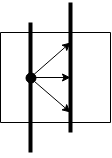
\includegraphics{img/Aperture}
	\caption{Example of aperture problem by the movement of a line.}
\end{figure}

On the other hand, if the texture is to structured, it may also bring uncertainty to the solution. If we take for example a sinusoidal wave like in \ref{apertureimgSin}, there is no telling if the signal moves up or down. As states in \cite{barron1994}, the authors encounter problems when testing the solutions based on SSD on such input sequences. Because of the periodical signal, the algorithms found more than one solution. As they made th search window bigger, the more (ghost as they called it) local minimas the algorithm found. 

\begin{figure}
	\label{apertureimgSin}
	\centering
	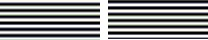
\includegraphics{img/sin}
	\caption{Example of aperture problem by the movement of a sinusoidal signal.}
\end{figure}


In optical flow, the simplest solution is the brightness assumption, that neighbouring pixels have the same movement.

\subsection{Lucas-Kanade}
Lucas-Kanade method solves the flow as a feature tracking algorithm. This differential method takes in account only the neighbourhood, solving for each pixel with last square estimation. From the brightness assumption, for a neighbourhood $\Omega$, the flow vector $[u_i,v_i]$ must satisfy: 
\begin{equation}
\begin{split}
	&I_x(x_1)+I_y(x_1) = - I_t	\\
	&I_x(x_2)+I_y(x_2) = - I_t \\
	&\vdots \\
	&I_x(x_n)+I_y(x_n) = - I_t 
	\end{split}
\end{equation} 

where $x_1$, $x_1$,  $...$,  $x_n$ are in the neighbourhood of pixel $i$.

Using the least square method, for each pixel in the image the energy function can be stated as:
\begin{equation} \label{gradientSumN}
	E(x) = \sum_{\substack{x \in \Omega}}
	 W^2(x)[\nabla I(x)\cdot \boldsymbol{v}+I_t(x)]^2
\end{equation}
where $W$ is a window function, Gaussian like, giving more weight to the canter pixel, rather than the neighbours.

To minimize $E(x)$, variational calculus is applied, and the derivatives of the equation \ref{gradientSumN} with respect to $u$ an $v$, respectively will be 0.

\begin{equation}
	\begin{split}
	\frac{\partial E}{\partial u} =  \sum_{\substack{x \in \Omega}}
	W^2(x)[I_x^2 u + I_x I_y v + I_x I_t] = 0 \\ 
	\frac{\partial E}{\partial v} =  \sum_{\substack{x \in \Omega}}
	W^2(x)[ I_x I_y u + I_y^2 v + I_y I_t]  = 0
	\end{split}
\end{equation}

If we demote
\begin{equation}
\begin{split}
A = \begin{bmatrix}
\nabla I(x_1), \ \dots , \ \nabla I(x_n)
\end{bmatrix} ^T \\
W = diag
\begin{bmatrix}
W(x_1), \ \dots , \ W(x_n)
\end{bmatrix}
\\
b = 
\begin{bmatrix}
-I_t(x_1), \ \dots, \ -I_t(x_n) 
\end{bmatrix}
\end{split}
\end{equation}
for each $n$ points $x_i \in \Omega$. Then, to minimize equation \ref{gradientSumN}, we differentiate  and the solution will be given by,
\begin{equation}
	A^T W^2 A  \boldsymbol{v} = A^T W^2 b 
\end{equation}
We multiplied the equation with $A^T$ on the left hand side, make the matrix nonsingular and be able to compute it's inverse. The Flow vector will be equal with:
\begin{equation}
\boldsymbol{v} = [A^T W^2 A  ]^{-1}A^T W^2 b
\end{equation}
where,

\begin{equation}
A^T W^2 A = 
\begin{bmatrix}
\sum W^2(x)I_x^2(x) \ \ \  
&\sum W^2(x)I_x(x) I_y(x) \\
\sum W^2(x)I_x(x) I_y(x) \ \ \  
&\sum W^2(x)I_y^2(x) 
\end{bmatrix}
\end{equation}
and
\begin{equation}
A^T W^2 b = 
\begin{bmatrix}
-\sum W^2(x)I_x(x)I_t(x)   \\
-\sum W^2(x)I_y(x) I_t(x)  

\end{bmatrix}
\end{equation}
 
by simple calculations we obtain
\begin{equation}
\begin{split}
	u =\frac{-\sum W^2I_y^2\ \sum W^2I_xI_t 
		+ \sum W^2I_x I_y  \sum W^2I_yI_t }
	{\sum W^2 I_x^2 \sum W^2 I_y^2
		- (\sum W^2 I_x I_y)^2 } \\
	u =\frac{\sum W^2I_x I_t\ \sum W^2I_xI_y 
		 - \sum W^2I_x^2  \sum W^2I_yI_t }
	{\sum W^2 I_x^2 \sum W^2 I_y^2
		- (\sum W^2 I_x I_y)^2 } \\
\end{split}
\end{equation}

\subsection{Correcting term}
As in the Lucas Kanade method, the flow equation can be solved, neglecting the aperture problem, as a local solution. But, as the window is getting bigger, the flow vector will be influenced by more neighbours, and the aperture problem is felt more as the results are more noisy. Why would one try to enlarge the system of equations? Well, because put it in a context and everything can change. By connecting the pixels with their neighbours, all te pieces will be connected and the system can be viewed as an ensemble. The results get better by solving the aperture problems. For example, as stated before, on surfaces with smooth, or no texture, the flow cannot be computed with a local method. But, if for a pixel in a textureless area, the flow is computed taking in account its neighbours, flow information will be propagated to it.

In addition to the brightness constraint, Horn and Schunk take a second term in equation, the smoothness constraint. The value of a pixel will be probably very close to its neighbours.

\begin{equation} \label{smoothEq}
	E_{smooth} = \iint (\left\Vert\nabla u \right\Vert_2^2 +\left\Vert\nabla v \right\Vert_2^2)dxdy
\end{equation}
where
\begin{equation}
	\nabla = \frac{\partial^2}{\partial x^2} + \frac{\partial^2}{\partial y^2}
\end{equation}
which means if the flow differs from a pixel to another (on $x$ and $y$ directions), the smoothness equation, \ref{smoothEq} will be high. As the algorithm tries to minimize the energy function\ref{HSEq}, the second term, \ref{smoothEq}, will also be minimized. If this term is closer to zero, the flow derivatives over $x$ and $y$  are smaller, which means the difference with the  neighbours is also smaller, in other words the flow is smooth.

The smooth term is more or less taken in account, depending on the nature of the input sequence. On some it works better with a higher weight, or in some, lower. Probably the best approach is to vary $\lambda$ weight of the second term in the flow equation \ref{HSEq}, and compare the results, like in a training stage of the program. Usually $\lambda$ is less than $1$ to avoid over smoothing.
\begin{equation}
	E = E_{data}+\lambda E_{smooth}
\end{equation}

To avoid this overall smoothing, as pixels may not be acting as a whole, $\lambda$ could be a matrix instead of a term, so each pixel can be influenced in his own percent of the neighbours.
An solution in computing this weight can be taken form the bilateral filter. The weight can be computed as explained in
\ref{bf}, so the smoothing term will influence each pixel differently. As when the pixel is on the edge, there should not be any influence from the neighbours, otherwise resulting in noisy results on the edges; but when the pixel is in the middle of an object, the velocity should ve influenced by its neighbours.

\section{Coarse-to-fine}
Differential methods cannot approximate large displacements. This is due to the small motion assumption. This problem can be solved with coarse-to-fine method.


 
Firstly, Gaussian Pyramids are built by successively blurring and unsampling into images of smaller and smaller resolutions. The unsampeling is done until the smallest resolution is about 30 pixels width or height.  Then, the flow is iteratively computed between each level of the pyramid, from the corest to the finest.
\subsection{Gaussian Pyramids}
The pyramid of an image is a multi-scale representation of it. In order to obtain the pyramids, successive smoothing and subsampling techniques are applied.  Each level is computed from the previous, recursively.


\paragraph{Building The pyramid} 
 Let us consider an image $I$ of size $m \times n$. The first level of the pyramid, the base is the image, $I_0$ is the image $I$, itself. The next level, $I_1$, is computed from $I_0$. The image $I_0$ is convoluted with a Gauss kernel, than the filtered image is sampled. $I_1$ is obtained with the dimensions $(m_0/sampling factor \times n_0/samplig factor)$. 

Similarly, the next levels are obtained, the $I_2$ is computed from $I_1$, $I_3$ from $I_2$, and so on.

Usually a sampling factor of $0.5$ is considered. If we consider $L$ the current level of the image, than we can obtain the $I_{L+1}$ image as fallows



\begin{equation} \label{eq1}
\begin{split}
I_{L+1}(x,y) = &\frac{1}{4}I_L(2x,2y)+\\
&\frac{1}{8}(I_L(2x-1,2y)+I_L(2x+1,2y)+I_L(2x,2y-1)+I_L(2x,2y+1))+\\
&\frac{1}{16}(I_L(2x-1,2y-1)+I_L(2x+1,2y+1)+I_L(2x-1,2y+1)+I_L(2x+1,2y-1) 
\end{split}
\end{equation}


\paragraph{Choosing the pyramid height}
As stated in the chapter before \ref{pyrHeight}, the height of the pyramids is usually chosen to have around 20-30 pixels on the height of the image, or width, respectively. The height is given by
\begin{equation}
	pyramid_{height} = \frac{\log\left(\frac{p}{\min(ht,wt)}\right)}
							{\log(d)}
\end{equation}
where p is the number of pixels on th top level on the minimum between  width $wt$ or the height $ht$.
\subsection{Warping the flow on the image}


At new level of the pyramid, the second image is warped to the first.
The new computed flow is considered.
Let us consider the current level $l$, and the computed flow $\boldsymbol{v}_l$, on the next level $l+1$, the second image is warped with the $\boldsymbol{v}_l$ velocities from the previous level.
At a certain level $l+1$ the warped image is 
\begin{equation}
I_w = interpolation(I_l, w_l+dw)
\end{equation}
where $w_l$ is the flow computed until the level $l$ and $dw$ the  residual flow computed at level $l$. Some algorithms, like proximal point approximation, do not compute the residual flow, but update directly the new flow.

\section{$L^2$ Solutions}
\subsection{Gauss-Seidel Iterations} \label{GaussSeidel}
Gauss Seidel is a iterative method for solving simultaneous equations.
\subsection{Jacobi Iterations}
\section{$L^1$ approach}

When the penalty function, $E(x)$ is of type $L^2$, like $\sigma(x)^2$,  the minimization problem is simple. One can reach the solution trough variational calculus, by differentiating the whole energy function with respect to $u$ and $v$, equalising with 0, and solving the system.  
For a faster convergence, some of the current algorithms use a $L^1$ penalty function, like modulus, others use a combination of both $L^2$ and $L^1$ penalty functions, for example, one for the data energy and one for the smoothness energy.

For this kind of formulations, the minimization can not be done any more trough differential techniques, and other approaches are used.

\section{other Improvements}
\subsection{Census transform}
\section{Error Measurement}
Now that the problem is stated, in order to get an idea of which behaves better on what conditions, we can compare the flow results with a ground truth. From Middlebury's website\cite{middleburry}, one can download their set of image sequences and the expected output. The images are artificially generated, so the flow between them is nearly the perfect result. This stands as a reference for the output of the algorithms, the errors are computed between this ground truth outputs and the results from the algorithms. Middlebury \cite{middleburry} also has a big database of the existing algorithms, classified by accuracy. Being referenced in most of the latest articles, it seems that this database is a good reference to modern approaches and their metrics.

\subsection{Cross correlation}

Cross correlation is a simple way to measure the difference between 2 signals.
\subsection{Endpoint error}
For measuring this error, the length of the vectors is taken in account. This error is expressed as the sum of differences both on the $x$ and $y$ directions, stated in a $L^2$ or $L^1$ norm.

\begin{equation}
\begin{split}
\sum  \sqrt{(u-u_{gt})^2+(v-v_{gt})^2} \\ 
\sum |u-u_{gt}|+|v-v_{gt}|
\end{split}
\end{equation}

Although the endpoint error can provide useful information about the vector's length, it contains no measurement of  the vector's orientation. To obtain this, the angular measurement is used.
\subsection{Angular error}
As we are talking about vectors, we need a complementary measurements over the magnitude error presented above.


\begin{equation}
\sum  \arccos \left( \frac{u^T \cdot u_{gt}}{|u||u_{gt}|}\right)
\end{equation}
 This error measurement is frequently used, as it evaluates both the magnitude and the direction of the flow. Of course, it has its downsides. By taking the magnitude in equation, the higher speeds have a greater impact on the final result then the lower speeds having the same angular error. 

\chapter{Proposed algorithm}

\chapter{Detailed Design and Implementation}

Together with the previous chapter takes about 60\% of the paper.

The purpose of this chapter is to document the developed application such a way that it can be maintained and developed later. A reader should be able (from what you have written here) to identify the main functions of the application.
\section{Derivative discretization}
\section{Sparse Matrix vs Iterative approach}
\section{Downsamplig and Pyramidal Implementation}
\section{Output and MATLAB Colorspace}
The chapter should contain (but not limited to):
\begin{itemize}
 \item a general application sketch/scheme,
\item a description of every component implemented, at module level,
\item class diagrams, important classes and methods from key classes.

\end{itemize}

\chapter{Testing and Validation}

About 5\% of the paper
\section{Title}
\section{Other title}

\chapter{User's manual}

In the installation description section your should detail the hardware and software resources needed for installing and running the application, and a step by step description of how your application can be deployed/installed. An administrator should be able to perform the installation/deployment based on your instructions.

In the user manual section you describe how to use the application from the point of view of a user with no inside technical information; this should be done with screen shots and a stepwize explanation of the interaction. Based on user's manual, a person should be able to use your product.

\section{Title}
\section{Other title}

\chapter{Conclusions}

About. 5\% of the whole

Here your write:
\begin{itemize}
\item a summary of your contributions/achievements,
\item a critical analysis of the achieved results,
\item a description of the possibilities of improving/further development.
\end{itemize}
\section{Title}
\section{Other title}


%\addcontentsline {toc}{chapter}{Bibliography} 
\bibliographystyle{IEEEtran} 
\bibliography{thesis}%same file name as for .bib

\appendix
\chapter{Relevant code}

\begin{verbatim}
Optimize (x,s,lambda)
\{
	D23SqInv = spdiags(1./ ...
				( ... 
					x(1+dim:2*dim)./s(1+dim:2*dim)+ ...
					x(1+2*dim:3*dim)./s(1+2*dim:3*dim)  ...
				) ...
				, 0, dim, dim);
	D23SqInv(isnan(D23SqInv)) = 0;
	
	D3 = spdiags(x(1:dim)./s(1:dim), 0, dim, dim);
	D2 = spdiags(x(1:dim)./s(1:dim), 0, dim, dim);
	D1Inv  = spdiags(s(1:dim)./x(1:dim), 0, dim, dim);        
	XInv = spdiags(1./x(:),0,3*dim, 3*dim);
	
	D3(isnan(D3)) = 0;
	D2(isnan(D2)) = 0;
	D1Inv(isnan(D1Inv)) = 0;
	XInv(isnan(XInv)) = 0;
	
	miu = mean(x(:).*s(:));
	sigma = std2(x(:).*s(:));
	ra = x(:).* s(:) - miu*sigma*ones(3*dim, 1);
	rc =  G*x+c-s-A'*l ;
	rb = A*x;
	rch =rc + XInv* ra;
	
	rch1 = rch(1:dim);
	rch2 = rch(1+dim:2*dim);
	rch3 = rch(1+2*dim:3*dim);
	
	rbh = rb + D2 * rch2 - D3 * rch3;
	rcTilda =rch1 +bfK'*(D23SqInv)*rbh;
	
	BigA = 2*G(1:dim, 1:dim)+D1Inv+bf2K'*D23SqInv*K;
	
	deltaF = gmres(BigA, -rcTilda);
	
	
	deltaL = D23SqInv*(-rbh-bfK*deltaF);
	deltaVp = D2*(-rch2-deltaL);
	deltaVm = D3*(-rch3-deltaL);
	deltaX = [deltaF; deltaVp; deltaVm];
	deltaS = G * deltaX- A'*deltaL+ rc;
	
	x = x + deltaX;
	s = s + deltaS;
	l = l + deltaL;
\}
\end{verbatim}

\chapter{Other relevant information (demonstrations, etc.)}
\section{Horn Scunk equation to Jacobi Iteration} \label{GSDemo}
First, let us define the staring equation.
\begin{equation}
	E = (I_xu+ I_yv + I_t)^2 + \lambda(\left\Vert(\nabla u) \right\Vert_2^2 +\left\Vert(\nabla v)\right\Vert_2^2)
\end{equation}
by discretizing $\left\Vert(\nabla u) \right\Vert_2^2$ with a Laplace filter, it can be rewritten as $(\bar{u}-u)^2$. The equation then becomes:
\begin{equation}
E = (I_xu+ I_yv + I_t)^2 + \lambda((\bar{u}-u)^2+(\bar{v}-v)^2)
\end{equation}
The we apply the partial derivatives and eqaual then to 0 in order to find the minimum, as E being convex,

\begin{equation} 
\begin{split} 
\frac{\partial E}{\partial u} = I_x(I_xu+I_yv+Iy) + \lambda(\bar{u}-u) \\
\frac{\partial E}{\partial v} = I_y(I_xu+I_yv+Iy) + \lambda(\bar{v}-v)
\end{split}
\end{equation}
Now to rearrange the  terms
\begin{equation} 
\begin{split} 
(I_x^2+\lambda)u + I_y I_x v  =  -I_xI_t + \lambda \bar{u} \\
I_y I_x u+(I_y^2+\lambda)v  = -I_yI_t + \lambda \bar{v} \\
\end{split}
\end{equation}
and in matrix form , $A \boldsymbol{x} = b$:

\begin{equation}
	\begin{bmatrix}
	I_x^2+\lambda & I_y I_x \\
	I_y I_x & (I_y^2+\lambda)
	\end{bmatrix}
	\cdot
	\begin{bmatrix}
	u \\
	v
	\end{bmatrix}
	=
		\begin{bmatrix}
	-I_xI_t + \lambda \bar{u}\\
	-I_yI_t + \lambda \bar{v}
		\end{bmatrix}
\end{equation}
The equation can be solved as $\boldsymbol{x} = A^{-1}b $. First to compute 
$A$'s determinant
\begin{equation}
	\frac{1}{\lambda(\lambda+I_x^2 + I_y^2)}
\end{equation}
the equation becomes:
\begin{equation}
\begin{bmatrix}
u \\
v
\end{bmatrix}
=
\frac{1}{\lambda(\lambda+I_x^2 + I_y^2)}
\begin{bmatrix}
I_y^2+\lambda & -I_y I_x \\
-I_y I_x & (I_x^2+\lambda)
\end{bmatrix}
\cdot
\begin{bmatrix}
-I_xI_t + \lambda \bar{u}\\
-I_yI_t + \lambda \bar{v}
\end{bmatrix}
\end{equation}

from this, on can easily find $u$ and $v$ as:
\begin{equation} \label{JEq}
\begin{split}
u^{k+1} = \frac{(I_{y}^2+\lambda)\bar{u}
	-I_{x}I_{y}\bar{v}
	-I_{x}I_{t}}{I_{x}^2+I_{y}^2+ \lambda}
\\
u^{k+1} = \frac{-I_{x}I_{y}\bar{u}
	+(I_{y}^2+\lambda)\bar{v}
	-I_{y}I_{t}}{I_{x}^2+I_{y}^2+ \lambda}
\end{split}
\end{equation}


\chapter{Published papers}

\end{document}
